\chapter{Discussion}

\begin{introduction}
    This chapter critically examines the developed Mixed Reality framework by discussing the key challenges encountered and outlining potential future applications in collaborative environments. While the implementation focused on achieving real-time, bidirectional communication and precise control of the UR10e robotic arm, numerous practical issues arose, primarily related to technical integration and ensuring synchronization between the physical and digital realms, leaving no time to perform user case studies.
\end{introduction}


\section{Challenges Faced During Implementation}
%  continue here
Though the development of the above described functionalities was successful, several challenges were encountered during the implementation phase that required substantial effort. The first hurdle was the integration of the robot’s digital model into the Unity environment using the Unity Robotics Hub's \texttt{URDF Importer} package. Unfortunately, an exact UR10e model was not available on-line, and a UR10 model was used instead~\footnote{PositronicsLab \url{https://github.com/PositronicsLab/reveal_packages/tree/master/industrial_arm/scenario/models/urdf/ur10} Accessed: 2024-02-05}. This change did not pose any dynamics problem, as the physical properties and kinematics between the two models are the same.

Ensuring accurate pose registration and alignment between the physical robot and its \ac{DT} in Unity presented a challenge. This required using a marker for precise \ac{AR} visualization. After testing several methods, the ArUco marker proposed in Figure \ref{f:aruco_marker} proved most effective for reliable tracking and better model alignment. Implementing this through Vuforia \ac{SDK} within Unity, along with relative positioning between the marker and digital model, was essential for maintaining synchronization between the physical and digital entities.

After having the digital model in the simulation environment, the correct position that would overlay it to the real robot had to be defined. This alignment proved to be difficult, since both the robot's digital model properties in Unity and its \ac{URDF} file required changes. These changes were performed via trial and error and an example of the disalignment can be seen in Figure \ref{fig:bigger-model}, were the \ac{DT} is clearly bigger and not superimposed to the real robot.

\begin{figure}[h]
    \centering
    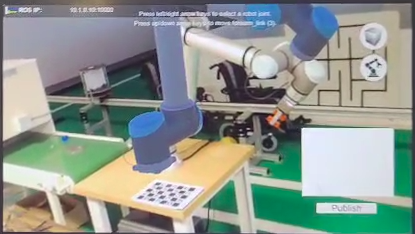
\includegraphics[width=0.7\linewidth]{figs/model-bigger.png}
    \caption{Disalignment example of the robot's digital next to the physical UR10e robot, within the Unity simulation environment. This offset is represented due to the scale disproportion between both entities.}
    \label{fig:bigger-model}
\end{figure}

During the development of the dissertation, testing was needed to ensure that the features would be working as supposed. In order to perform these tests, the Unity simulation had to be running on a laptop, since the Unity application would only be built into the \ac{HHD} in the dissertation's development final stage. Therefore, it was crucial to properly visualize the robot's surrounding environment, which was done with the camera shown in Figure \ref{fig:camera-c922}. Due to the distance required to view the \ac{AR} marker that would lay the robot's digital model in the environment and perform posterior analysis of the feature that was being tested, this methodology proved to be ineffective given that the laptop and its connected \ac{USB} camera would need to be constantly moved around to track the whole environment. Figure \ref{fig:holding-camera} depicts a solution to this issue, where another person helps testing the developed features by holding the camera in a static position.

\begin{figure}[h]
    \centering
    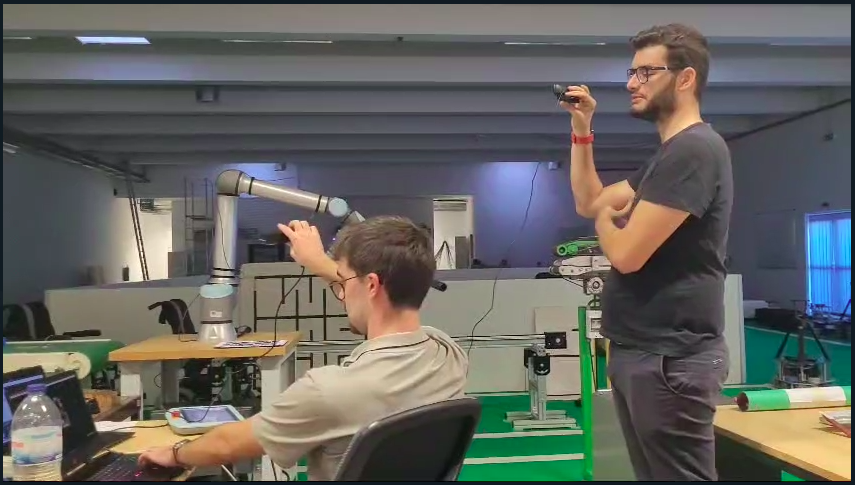
\includegraphics[width=0.7\linewidth]{figs/eu-ze.png}
    \caption{Testing setup for the \ac{MR} application, where an assistant holds a camera to capture the robot's surrounding environment. This method allowed for better tracking of the \ac{AR} marker, ensuring an alignment of the robot’s \ac{DT} for posterior features' tests. Due to the need for precise marker visibility, this setup presented a solution to the need of constantly repositioning the laptop and its \ac{USB} connected camera around the environment.}
    \label{fig:holding-camera}
\end{figure}

% practical issues arose during testing, as the camera and laptop needed to be moved frequently to maintain proper marker alignment.

When establishing the bidirectional communication between the \ac{ROS} middleware and the Unity \ac{MR} environment, the Unity Robotics Hub repositories played a critical role~\footnote{\url{https://github.com/Unity-Technologies/Unity-Robotics-Hub}, Accessed: 2024-10-29}. Integrating these tools was not straightforward due to the lack of comprehensive documentation, particularly around generating and handling \ac{ROS} messages from within Unity’s \texttt{C\#} environment. \ac{ROS} messages needed to be generated, transmitted, and handled effectively, but interfacing between \texttt{C\#} and \ac{ROS} message types such as \texttt{JointState.msg} proved challenging. All \ac{ROS} \texttt{sensor\_msgs}~\footnote{\url{https://wiki.ros.org/sensor_msgs}, Accessed: 2024-10-29} had to be included into the Windows environment to be properly built within Unity, as depicted in Figure \ref{fig:unityjoint_state_message}. Moreover, managing \ac{ROS} messages within Unity’s \texttt{C\#} environment required significant effort in order to ensure proper serialization and deserialization. Once the messages were correctly generated on the Unity side, the robot's joint states were transmitted from \ac{ROS} and saved as a \texttt{JSON} file in Unity. This \texttt{JSON} file was then used to update the \ac{DT} in real-time, maintaining the synchronization between the physical robot and its virtual counterpart. The reverse process, where joint coordinates are sent from Unity to \ac{ROS}, also posed difficulties due to the complexity of publishing these messages back to the \ac{ROS} environment. This step was crucial to ensure that changes made in the Unity \ac{MR} environment could correctly influence the physical robot, reinforcing the \ac{DT} concept's importance.

\begin{figure}[h]
    \centering
    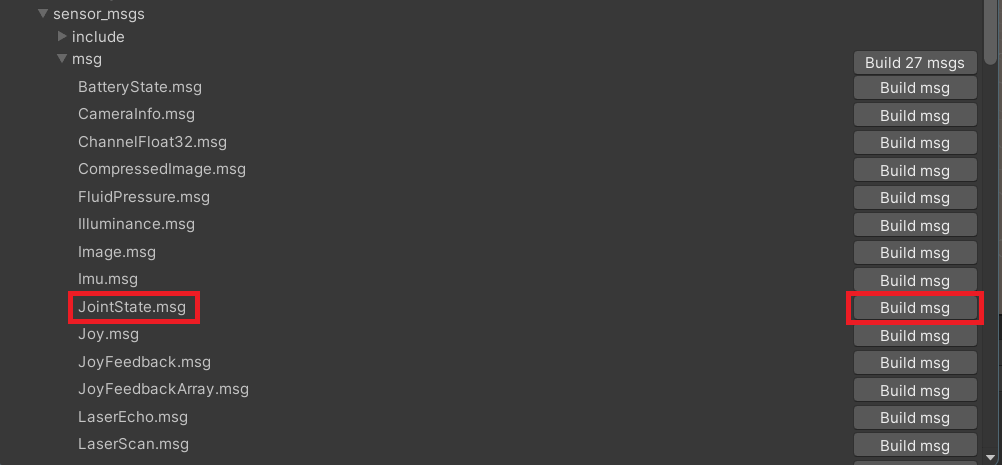
\includegraphics[width=0.7\linewidth]{figs/unityjoint_state_message.png}
    \caption{JointState message generation in Unity, corresponding to the desired ROS message}
    \label{fig:unityjoint_state_message}
\end{figure}

One additional challenge was the live camera feed transmission from \ac{ROS} to Unity, which proved to be too large to transmit efficiently over the network, resulting in significant latency. To address this, the image data had to be compressed using the \texttt{image\_transport} package in \ac{ROS}, which allowed the camera feed to be republished in a more compact format. This enabled real-time transmission over a \ac{TCP}/\ac{IP} connection, ensuring that the remote user could observe the robot’s workspace without excessive delay.

By the time all the developed features were working properly, building the Unity-based \ac{MR} application for deployment on a \ac{HHD} presented significant challenges. There are no certainties regarding where do these issues come from, however, integrating several packages essential for achieving robotics bidirectional communication, precise model rendering and manipulation within Unity, could have affected the deployment and runtime stability of the application on mobile devices.

In conclusion, while the implementation of the core functionalities of the \ac{MR} application—such as robot control, bidirectional communication, and user interface elements—was successful, the project encountered significant obstacles mainly related to the lack of documentation, support and examples that enables the integration of external tools and the handling of \ac{ROS} messages in Unity. This lack of resources complicated the development process, yet the solutions developed play a foundational role and offer substantial value to the community. By implementing core funcionalities like robot control with bidirectional communication and \ac{UI} features integration, this dissertation enables future advancements, such as robust system testing and performance evaluations. Despite not having conducted a user testing, the framework serves as a valuable platform for further exploration and validation of \ac{MR} based \ac{DT} integrated applications in \ac{HRC}.



\section{Scenarios of Relevant Future Use-Cases}

The developed \ac{MR} system could be applied to a wide range of collaborative tasks involving \ac{HRI}. Core functionalities of the system include using a \ac{DT} to ensure synchronization between the physical robot and its virtual counterpart, allowing both co-located and remote members to control and monitor the robot in real-time. The live camera feed from the robot provides additional visual context for remote experts, enabling precise instructions and adjustments during complex tasks. Safety zones are implemented to ensure that on-site operators can interact safely with the robot, halting operations if predefined zones are breached. For example, in an assembly task, the on-site user and the remote expert can work together using a robotic arm, aided by the system’s \ac{MR} interface. This enables both users to visualize the workspace and the robot’s actions in real-time, enhancing their collaborative decision-making. 

Despite the challenges aformentioned, the proposed system has potential to be relevant in various areas of application. Below, some examples are given, helping ilustrate where the developed features can have a significant role in \ac{HRC} supported by \ac{MR} and robotics, such as industries like automotive/electronics assembly and healthcare, where precision and real-time collaboration are essential. The remote expert could guide on-site technicians in performing intricate tasks while maintaining full visibility of the robot’s actions through the \ac{MR} interface. However, regarding ergonomics and safety features, these would need to be tailored to industry-specific needs, ensuring that the system promotes both efficiency and user well-being.

One relevant use case, paramount in industries worlwide, is related to assembly scenarios. The \ac{MR} system could facilitate collaboration between an on-site technician and a remote expert during a complex assembly task such as an airplane's engine. The on-site user arranges the engine's pieces while the remote expert guides the process via the \ac{MR} interface, visualizing the robot’s workspace and controlling the UR10e robotic arm. While the on-site user positions larger components, the remote user, viewing the real-time camera feed and \ac{DT} synchronization, handles intricate placements with precision. Both users interact with the robot using the \ac{MR} interface, allowing seamless handoffs and clear coordination. Virtual safety zones ensure that on-site members are protected from accidental robot movements. This application highlights how the system could be used to improve teamwork, task accuracy, and efficiency in precise, component-based tasks, with the real-time updates and collaboration capabilities ensuring minimal errors during assembly.

Another relevant are of application envisioned for the proposed system is healtcare. The \ac{MR} system could be deployed to assist in a remote surgical procedure. An on-site surgeon collaborates with a remote expert who oversees the operation via the \ac{MR} interface. The robotic arm assists with precise movements during surgery, such as handling instruments or holding tissues. Again, the live camera feed from the robot provides the remote expert with a surgeon’s view of the operation, while the \ac{DT} in the \ac{MR} interface mirrors the robot's real-time movements. The remote expert can adjust the robot’s actions, guiding the on-site surgeon through critical parts of the procedure. Gesture-based interactions can further enhance communication between the two users, allowing natural, intuitive commands during surgery. Here, the system can enhance precision, reduce risk, and facilitate collaboration between geographically distant medical professionals in high-stakes environments like surgeries.








% *TODO: explain this part of the use case scenario better - improve it
% A detailed application scenario for the developed \ac{MR} application could involve a collaborative LEGO assemly task, where an on-site operator and a remote expert work together to assemble a complex LEGO structure using the UR10e robotic arm.

% The on-site user initiates the task by organizing the workspace and placing the necessary LEGO pieces. The remote expert, using the developed \ac{MR} interface, connects to the environment and visualizes both the workspace that the on-site member is sharing as well as the robot’s perspective through the live camera feed. Both users can interact with the robotic arm in real-time. While the remote user can only do it via the \ac{MR} interface, the on-site user can also manipulate the real robot either directly through the \ac{MR} interface or by issuing commands via the \ac{ROS} middleware, depending on the complexity of the task.

% % \subsection{Collaborative Process}

% The \ac{DT} robot in Unity environment mirrors the on-site robot's physical actions, allowing the remote user to understand the real-time state of the robot. The remote user can identify specific LEGO pieces and their placements by observing the robot's workspace in real-time, provided by the camera live feed. Through the \ac{MR} interface, the expert manipulates the \ac{DT}, being able to publish the desired positions into the real robot. 

% % Task Coordination:
% The on-site user may position larger LEGO blocks or prepare specific segments of the structure, while the remote user takes control of the more precise and intricate assembly steps. The real-time updates of the DT and bidirectional communication allow the robot to switch seamlessly between both users’ inputs, ensuring accurate piece placement and synchronization of actions.

% % Utilization of Safety and Control Features:

% To ensure user safety during this collaborative assembly task, virtual safety zones surrounding the robot's working area are activated. These zones prevent the robot from moving too close to the on-site user and in case the user accidentally breaches these zones, the robot will halt its movement and auditory alerts would sound. This feature enhances the safety of the interaction, preventing potential accidents during the task.

% % Control Methods:
% % Three control modes enhance this task's flexibility. The on-site user may utilize the UI control for manual, direct adjustments to the robot’s movements, whereas the remote expert can use the Unity-ROS control method to command precise joint movements from their location. Both users have synchronized perspectives, thanks to the camera feed and DT updates, allowing them to work efficiently without unnecessary delays.


% *TODO: refine this example case
% An example case could involve using the system in an automotive assembly process. In this scenario, a remote expert guides the on-site technician through \ac{AR} during complex assembly tasks, offering real-time feedback and instructions. Furthermore, the system could monitor the worker’s movements, providing feedback on ergonomics to ensure proper posture and technique, reducing the risk of injury.
% By assessing the impact on assembly time, error rates, and productivity over an extended period, this study could yield valuable insights into both individual and collaborative task performance. This investigation would also explore how prolonged \ac{AR} device usage affects user comfort, preventing issues like fatigue, cognitive overload, or physical strain. Technicians’ interactions with \ac{AR} tools such as the HoloLens 2 would be closely evaluated, ensuring sustained comfort and efficiency in real-world industrial settings.


% % use case scenario - change it
% \section{Use Case Scenario: Collaborative Robot-Assisted Assembly Task}
% \label{sec:use_case}

% To validate the application developed in this project, we propose a practical use case scenario in which a human-robot collaborative system is used to assist in a real-time assembly task. The scenario involves a remote user and an on-site operator working together to assemble a complex product, such as a LEGO structure, using the robotic arm UR10e to perform precise tasks like identifying, picking, and placing components.

% \subsection{Assembly Task Description}
% The task requires the human operator and the robotic arm to collaborate in assembling various parts of the product. The on-site user prepares the workspace by organizing components and configuring the robot, while the remote user oversees the assembly process and directly controls the robot's movements via the \ac{MR} interface. The robot, equipped with a mounted camera, captures a live video feed of the workspace, streamed to the remote participant in real time. This video allows the remote user to see exactly what the robot is observing, thus ensuring precise actions for component identification, manipulation, and placement.

% \subsection{Features Utilized in the Assembly Process}

% \begin{itemize}
%     \item \textbf{On-Site and Remote Collaboration:} The \ac{MR}-based system allows both the on-site and remote users to collaboratively control and monitor the robot’s actions. The on-site operator can use the developed \ac{HHD} interface for fine-tuning the robot’s movements, while the remote user manipulates the robot using the virtual interface, synchronizing real-world and digital movements.
    
%     \item \textbf{Digital Twin (\ac{DT}) Synchronization:} The \ac{DT} of the UR10e, aligned through Vuforia using ArUco markers, ensures that both the remote and on-site members are consistently aware of the robot’s state. Any movement of the robot, either from remote commands or physical interactions, is accurately mirrored in the Unity-based \ac{MR} interface.

%     \item \textbf{Real-time Video Streaming:} The live camera feed mounted on the UR10e arm streams a real-time video of the robot’s workspace to the remote user, providing full visual context of the assembly task. This reduces the burden on the on-site operator to manually share visual information, allowing the remote user to have a direct perspective of the task and make adjustments as needed.

%     *TODO: correct this part 
%     \item \textbf{Safety Zones:} Despite the developed virtual safety zones, displayed in the \ac{MR} interface, being more relevant for the on-site user to prevent collisions during robot operation, these can be easily modified regarding the use-case scenario described. Instead of halting its movement if the on-site member enters the robot working area, visual and auditory alerts are triggered, improving the safety of the interaction. The robot will automatically halt if it detects an on-site user breaching the predefined zones, preventing potential accidents.

%     \item \textbf{Bidirectional Control and Feedback:} The bilateral communication established through ROS-TCP Connector allows commands from the remote user to be executed in real time by the robot, and the robot’s state is reflected back to the digital environment. This ensures that the robot follows precise trajectories, and real-time feedback from the ROS environment ensures synchronization between the virtual and physical models.

%     \item \textbf{Camera Feed Transmission:} The camera feed enhances situational awareness for the remote participant, who can directly monitor the assembly process through the robot’s perspective. This feature reduces the cognitive load on the on-site operator, enabling the remote user to make real-time decisions regarding component handling and placement, ultimately improving task efficiency.

% \end{itemize}

% \subsection{Potential Industrial Applications}

% This human-robot collaborative system has wide-ranging applications in several industries that rely on precise assembly tasks:

% \begin{itemize}
%     \item \textbf{Electronics Manufacturing:} In industries such as electronics manufacturing, where delicate components need to be assembled with high precision, the system could be applied to remotely assemble small and fragile parts. The real-time video feed and \ac{MR} interface would ensure that the remote operator has full visibility of the workspace, while the robot performs tasks requiring high precision, like picking and placing tiny components.

%     \item \textbf{Automotive Assembly:} In automotive production, remote technicians could assist on-site workers in installing or assembling complex parts. For example, during the assembly of engines or electric vehicle batteries, the robot could handle heavy or dangerous components while the human operator provides real-time guidance from a safe distance.

%     \item \textbf{Aerospace Component Assembly:} Aerospace applications often involve complex, high-value assemblies where precision is critical. The collaborative system could enable engineers to remotely guide robotic arms to fit components with tight tolerances, reducing human error and improving task consistency.

%     \item \textbf{Medical Device Manufacturing:} In medical device manufacturing, this system could ensure the safe and precise assembly of small, intricate parts, where any mistake could be costly. Remote experts could oversee the assembly process, while robots assist in handling and assembling the delicate components of surgical instruments or diagnostic devices.

% \end{itemize}

% \subsection{Advantages of the System}
% The integration of the developed \ac{MR}-based system into such industrial applications offers several advantages:

% \begin{itemize}
%     \item \textbf{Enhanced Remote Collaboration:} The real-time synchronization between the digital twin and physical robot, combined with live camera feeds, allows remote experts to have full control over assembly tasks without being physically present, enabling global collaboration.
    
%     \item \textbf{Improved Efficiency and Precision:} The ability to delegate repetitive or precision-dependent tasks to the robot, while the human focuses on higher-level decision-making, improves overall task efficiency. The \ac{MR} interface provides a more intuitive control mechanism than traditional robotic interfaces.
    
%     \item \textbf{Safety:} The implementation of virtual safety zones and real-time feedback mechanisms ensures that human workers remain safe while working closely with robots. This reduces the risk of accidents in high-risk environments such as automotive and aerospace manufacturing.

%     \item \textbf{Cost-Effective and Scalable:} By enabling remote operation, the system reduces the need for on-site presence, minimizing travel costs and downtime. It is also scalable across multiple sites, allowing experts to manage operations in various locations without needing to be physically present.

% \end{itemize}

% In summary, this use case scenario illustrates the practical value of the developed features in collaborative human-robot assembly tasks. The combination of real-time robot manipulation, live video streaming, and digital twin synchronization offers a powerful toolset for modern industrial environments, enhancing productivity, safety, and collaboration.
